% !TeX root = ../../Skript.tex
\cohead{\Large\textbf{Schnittstellen und Schnittpunkte}}
\fakesubsection{Schnittstellen und Schnittpunkte}
Erinnerung: In der Mathematik unterscheidet man grundsätzlich zwischen Stellen und Punkten. Stellen sind x-Werte während Punkte einen x-Wert und einen y-Wert haben. Die Schnittpunkte zweier Funktionen \(f(x)\) und \(g(x)\) sind alle Punkte, in denen sich die Schaubilder schneiden. Um die Schnittstellen zu erhalten, muss man die Funktionen gleichsetzen:
\begin{tcolorbox}\centering
	\(\textcolor{loestc}{f(x)=g(x)}\)
\end{tcolorbox}

\begin{minipage}{\linewidth}
	\adjustbox{valign=t, padding=0ex 0ex 2ex 0ex}{\begin{minipage}{0.5\linewidth-2ex}
			\iftoggle{ausfuellen}{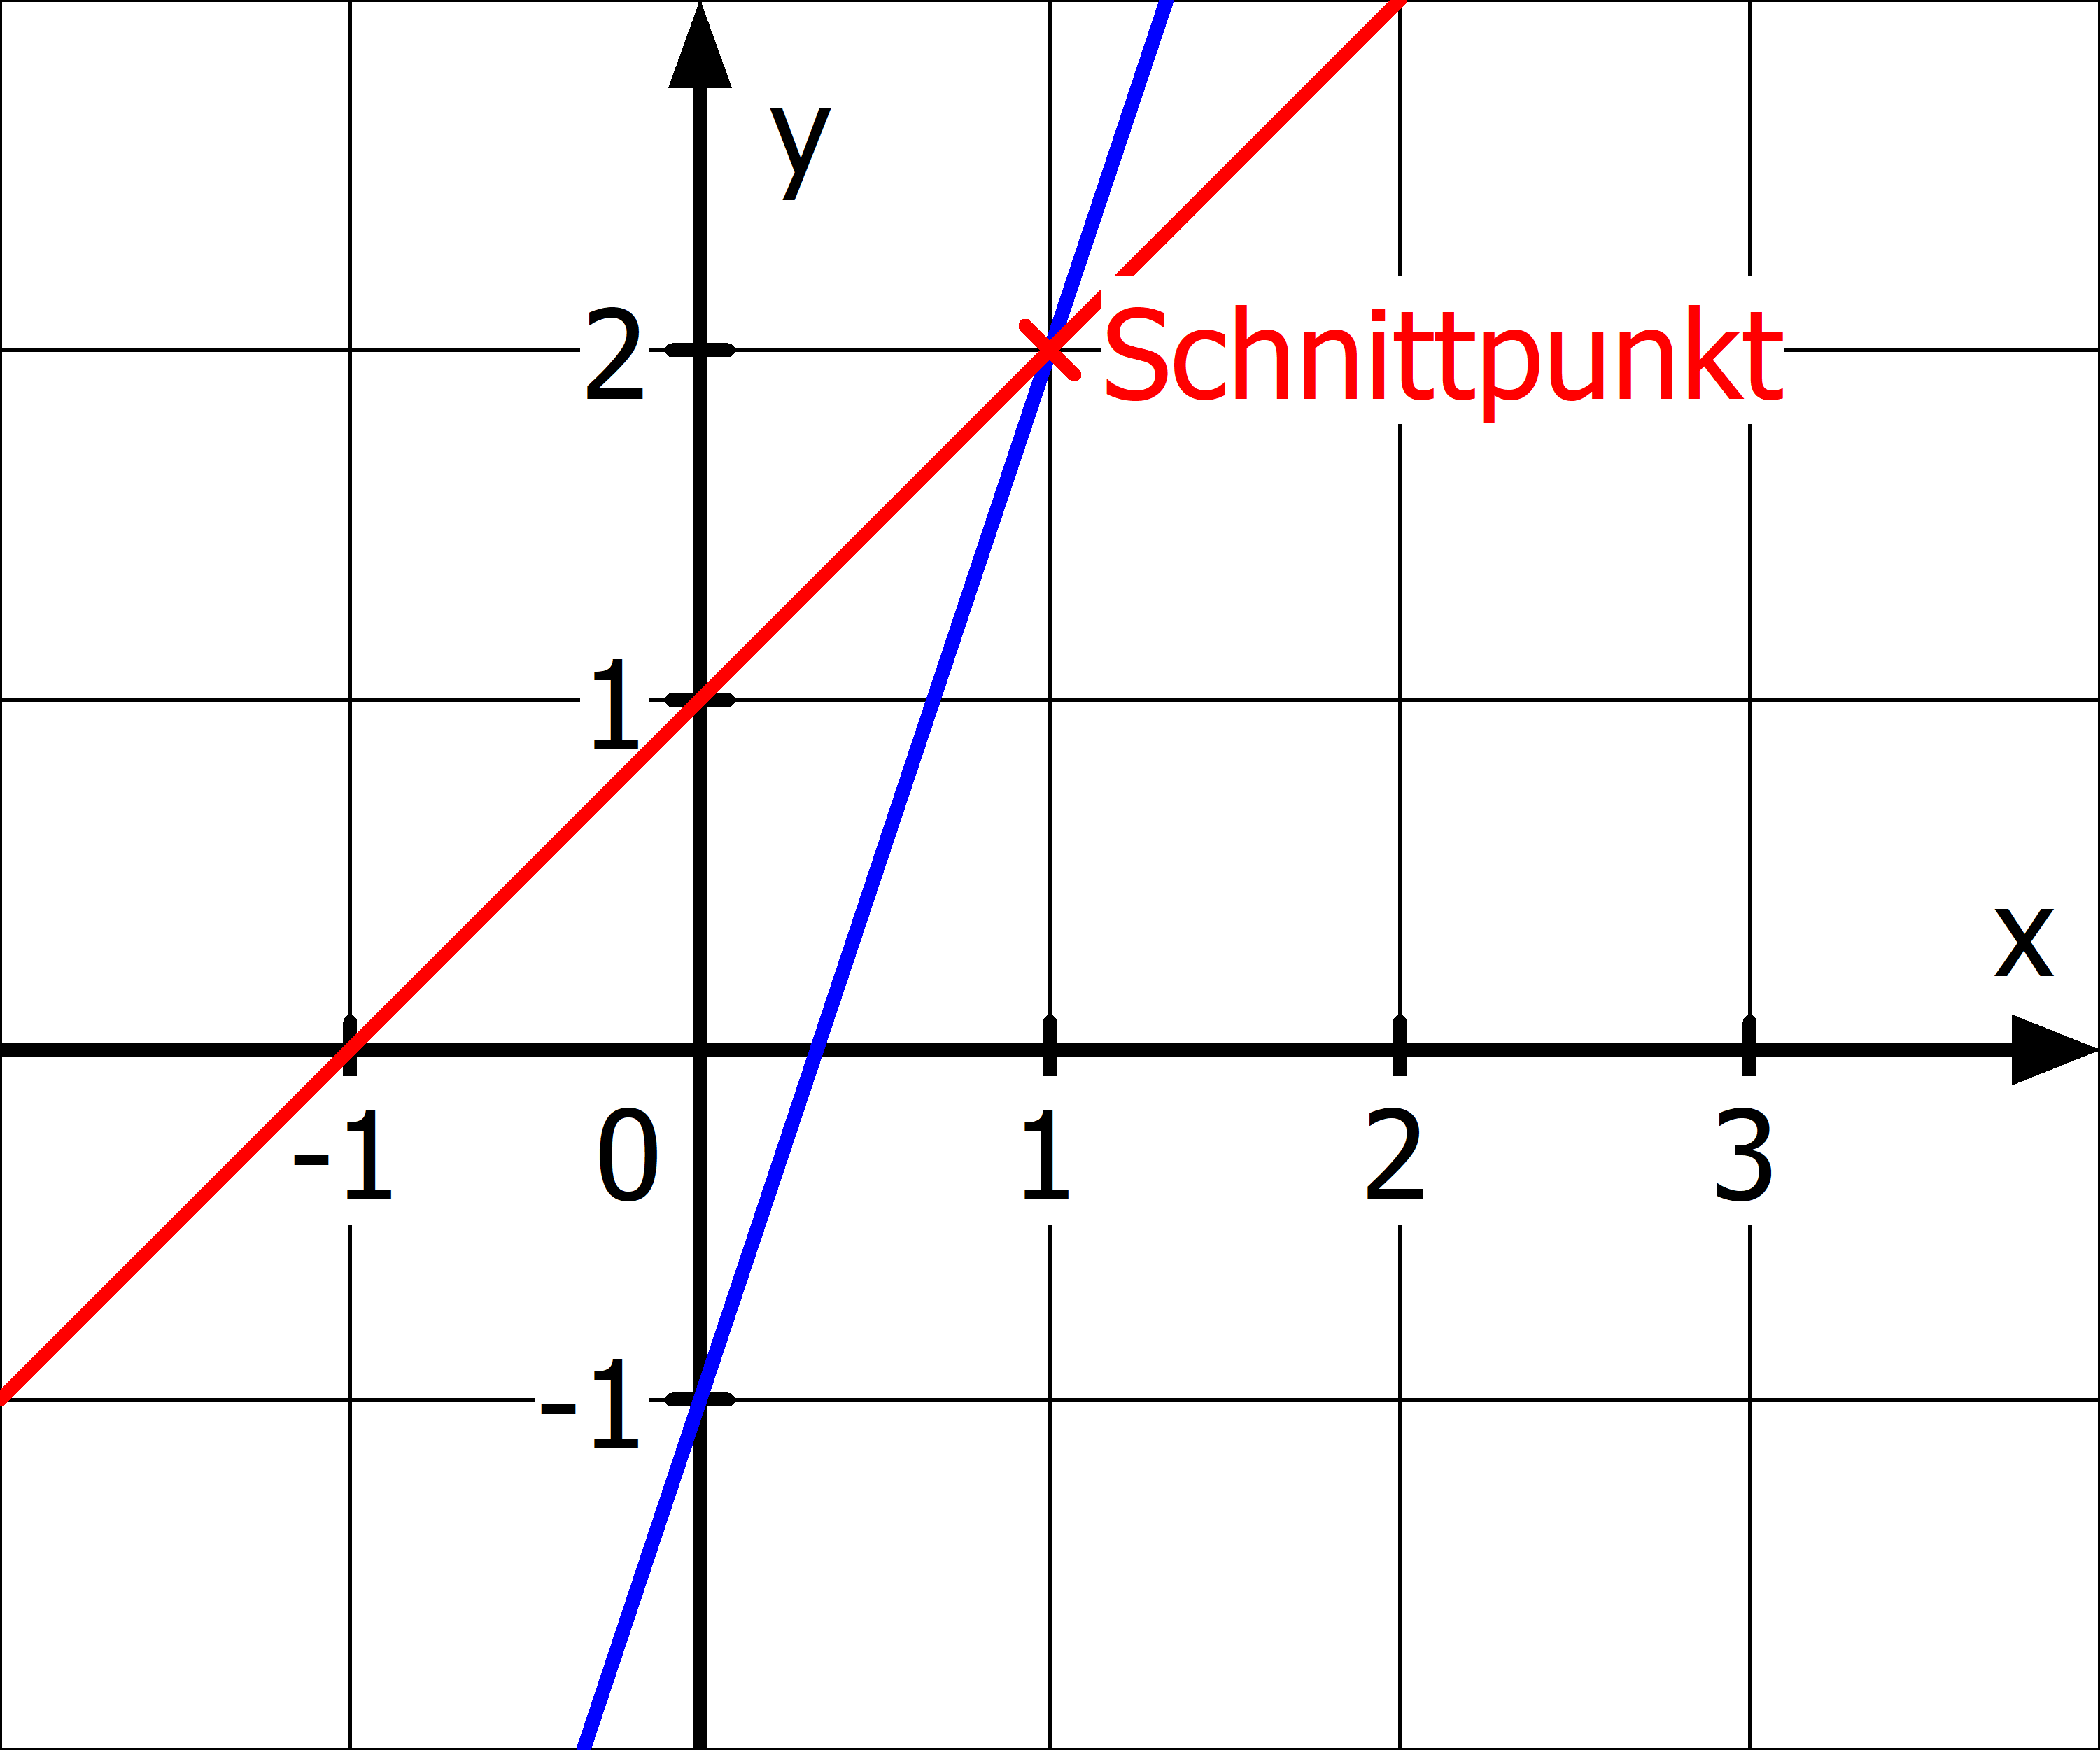
\includegraphics[width=\linewidth]{\linFkt/pics/schnittpunkt.png}}{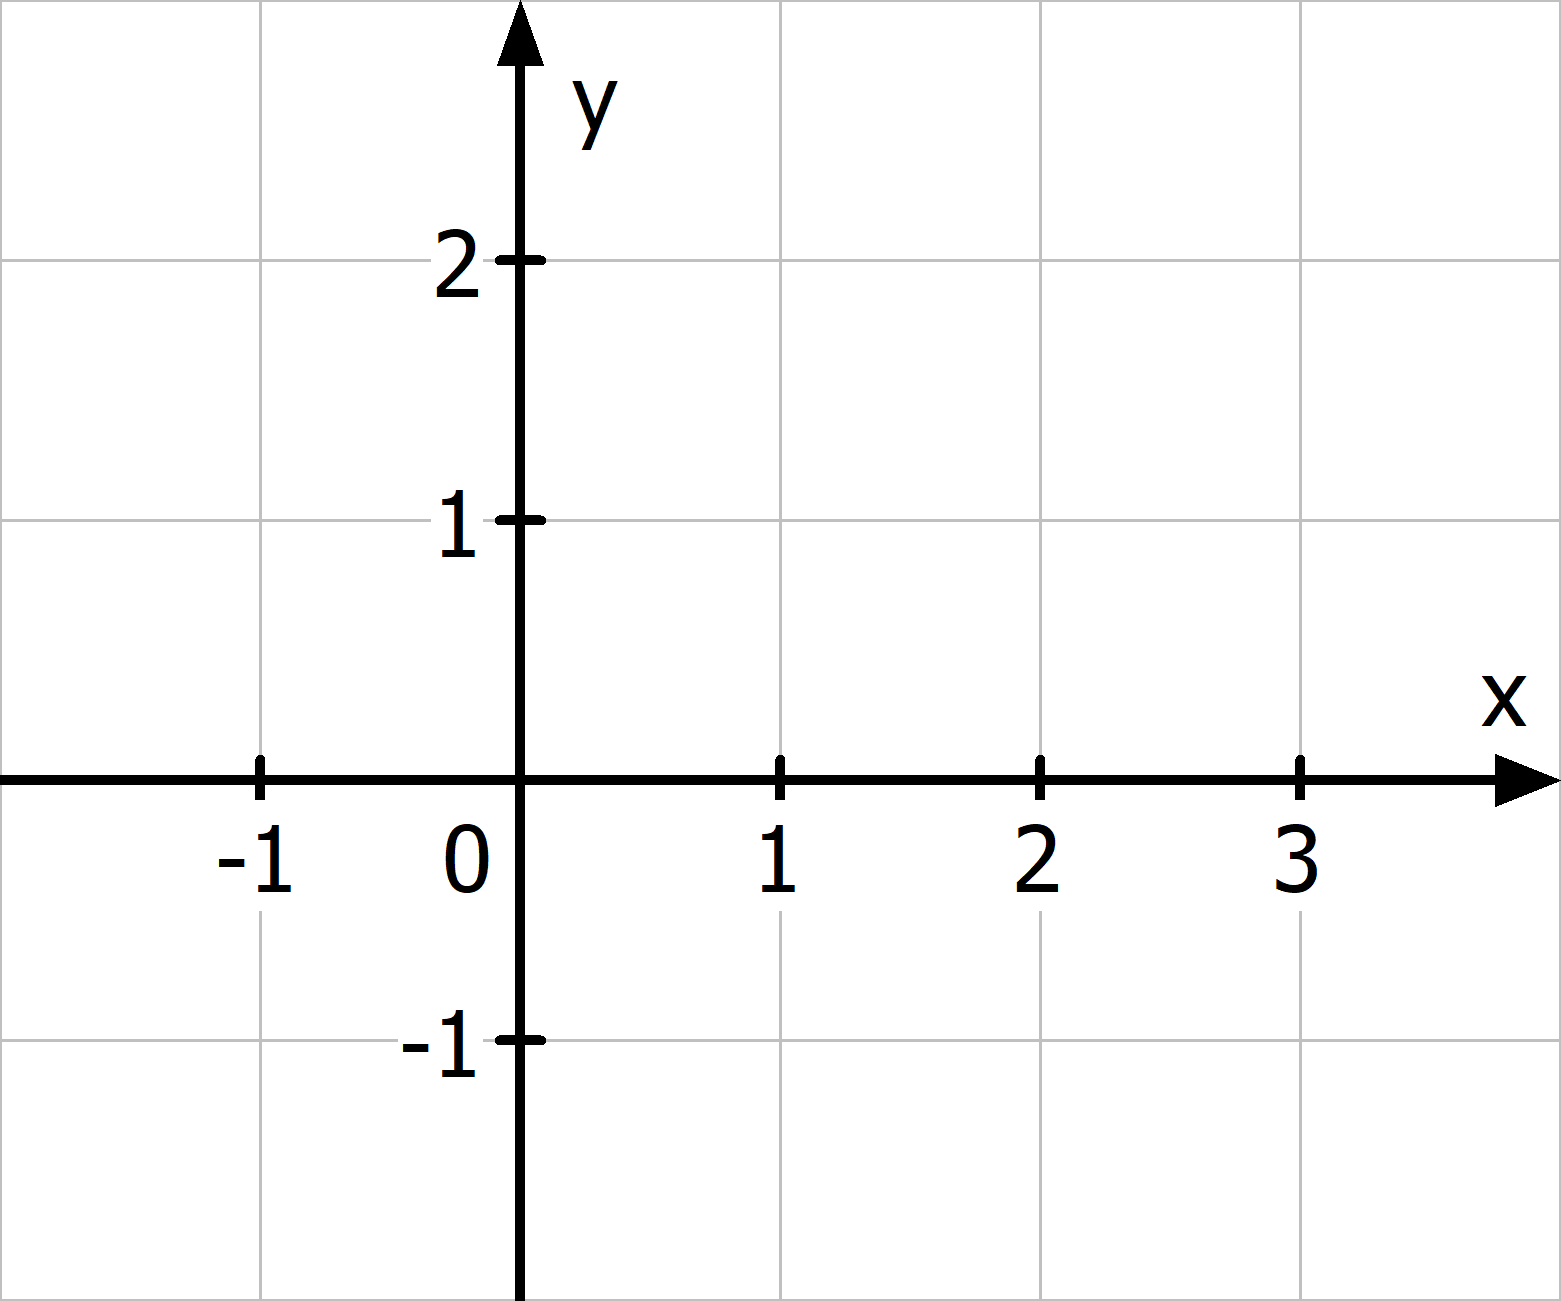
\includegraphics[width=\linewidth]{\linFkt/pics/schnittpunkt_empty.png}}
	\end{minipage}}%
	\adjustbox{valign=t, padding=2ex 0ex 0ex 0ex}{\begin{minipage}{0.5\linewidth-2ex}\raggedright
			Im nebenstehenden Beispiel sind die Schaubilder der Funktionen \(\textcolor{red}{f(x)=x+1}\) und \(\textcolor{blue}{g(x)=3x-1}\) gezeichnet. Der Schnittpunkt lässt sich wie folgt berechnen:
			\begin{align*}
				\textcolor{loes}{f(x)}&\textcolor{loes}{\;=g(x)}\\
				\textcolor{loes}{x+1}&\textcolor{loes}{\;=3x-1\ \vert -3x-1}\\
				\textcolor{loes}{-2x}&\textcolor{loes}{\;=-2\ \vert \cdot\left(-\tfrac{1}{2}\right)}\\
				\textcolor{loes}{x}&\textcolor{loes}{\;=1}
			\end{align*}%
	\end{minipage}}%
\end{minipage}%

\bigskip

Die Schnittstelle ist also \(\textcolor{ForestGreen}{x=1}\). Um die y-Koordinate zu erhalten, setzt man \(\textcolor{ForestGreen}{x=1}\) entweder in \(\textcolor{red}{f(x)}\) oder \(\textcolor{blue}{g(x)}\) ein. Zur Demonstration setzen wir die Schnittstelle in beide Funktionen ein:
\begin{align*}
	\textcolor{red}{f(}\textcolor{ForestGreen}{1}\textcolor{red}{)}&=\textcolor{red}{\textcolor{ForestGreen}{1}+1}=\textcolor{YellowOrange}{2}\\
	\textcolor{blue}{g(}\textcolor{ForestGreen}{1}\textcolor{blue}{)}&=\textcolor{blue}{3\cdot \textcolor{ForestGreen}{1}-1}=\textcolor{YellowOrange}{2}
\end{align*}
Der Schnittpunkt liegt also bei \(P\left(\textcolor{ForestGreen}{1}\middle\vert\textcolor{YellowOrange}{2}\right)\).
\begin{Exercise}[title={Bestimme jeweils den Schnittpunkt}, label=schnittpunktA1]

	\begin{minipage}{0.5\textwidth}
		\begin{enumerate}[label=\alph*)]
			\item \(f_1(x)=x-1\text{ und }g_1(x)=-x+3\)
			\item \(f_2(x)=-2x+4\text{ und }g_2(x)=0,5x-1\)
			\item \(f_3(x)=\frac{3}{2}x+\frac{1}{2}\text{ und }g_3(x)=4x\)
		\end{enumerate}
	\end{minipage}%
	\begin{minipage}{0.5\textwidth}
		\begin{enumerate}[label=\alph*)]
			\setcounter{enumi}{3}
			\item \(f_4(x)=\frac{4}{5}x+\frac{2}{5}\text{ und }g_4(x)=-\frac{2}{5}x\)
			\item \(f_5(x)=-\frac{2}{3}x-15\text{ und }g_5(x)=3x-\frac{5}{4}\)
			\item \(f_6(x)=-\frac{5}{8}x\text{ und }g_6(x)=-\frac{3}{2}x+\frac{1}{2}\)
		\end{enumerate}
	\end{minipage}%
\end{Exercise}\vspace{.5cm}
\begin{Answer}[ref=schnittpunktA1]\\
	\begin{minipage}{0.5\textwidth}
		\begin{enumerate}[label=\alph*)]
			\item \(P_1\left(2\middle\vert 1\right)\)
			\item \(P_2\left(2\middle\vert 0\right)\)
			\item \(P_3\left(\frac{1}{5}\middle\vert \frac{4}{5}\right)\)
		\end{enumerate}
	\end{minipage}%
	\begin{minipage}{0.5\textwidth}
		\begin{enumerate}[label=\alph*)]
			\setcounter{enumi}{3}
			\item \(P_4\left(-\frac{1}{3}\middle\vert \frac{2}{15}\right)\)
			\item \(P_5\left(-\frac{15}{4}\middle\vert -\frac{25}{2}\right)\)
			\item \(P_6\left(\frac{4}{7}\middle\vert -\frac{5}{14}\right)\)
		\end{enumerate}
	\end{minipage}%
\end{Answer}